\documentclass{article}

\title{P01-Malloc Report}
\date{19/10/2017}
\author{150008859}

\setlength{\parskip}{1em}
\setlength{\parindent}{0em}

\usepackage{listings}
\usepackage{amsmath,amssymb,amsthm}
\usepackage{mathtools}
\usepackage{graphicx}

\usepackage{graphicx}
 

\lstset{language=C}

\begin{document}
\maketitle
\newpage

\section{Introduction}

Before I started this practical, I researched existing memory allocators. In particular, I was intrigued by Glibc Malloc. Glibc Malloc originated as a fork of Doug Lee's memory allocator with support for multithreading. Originally named ptmalloc2, after being adapted into and maintained as a part the glibc library, it was referred to as Glibc Malloc \cite{sploitfun}.

In this report, I present an overview of my memory allocator, of which most the ideas and data structures are directly inspired by and present in Glibc Malloc source code \cite{malloc} or any of the 3 sources describing memory allocators below.

\section{Usage}

I included two (functionally identical) copies of my practical.

The folder ``P1-Malloc-stackscheck'' works with stackscheck (and its Makefile).

The folder ``P1-Malloc-readable'' contains code that is modular and readable.

\section{Data Structures}

Two of the most important algorithms used in memory allocators are Boundary Tags and Binning \cite{douglee}. In this report, I refer to free lists as bins. 

\subsection{Chunks}

\begin{lstlisting}
  struct chunk {
    size_t psize; /* Previous Size or Last 8 bytes of user controlled memory */
    size_t csize; /* A multiple of 8, so last 3 bits store meta data */
    struct chunk *next; /* Free List ptrs Or ... */
    struct chunk *prev; /* ... User Controlled Memory */  
  };
\end{lstlisting}

A Chunk is a header of its piece of memory and the footer of the piece of memory behind it.

The chunk size (csize) of a chunk is a multiple of 8 bytes, so we can use the last 3 bits in csize to chunk meta data. 

\begin{tabular}{ c | c }
  Bit & If this bit is set \\ \hline	
  0 & The previous chunk is use. \\
  1 & This a directly mmaped chunk. \\
  2 & This chunk belongs to a non-main arena \\
\end{tabular}

If the previous chunk is free, then the previous size (psize) member stores the previous chunk's size. Psize represents the last 8 bytes of user controlled memory, hence if the previous chunk is not free, it will contain user data. In use chunks are not tracked. 

Therefore, this data structure is header of the current chunk and the footer of the previous chunk (by storing the size of the previous chunk) which in practice means it supports boundary tags. Boundary tags are important for traversing chunks forwards and backwards and for coallescing adjacent free chunks to minimise fragmentation \cite{douglee}. 

Finally, a chunk contains pointers to a next and prev chunk so it can be stored in a circular doubly linked free list. A non-free chunk would otherwise contain user data in this region of memory.

\begin{figure}[!htb]
\caption{A graphic of a chunk taken from \cite{sploitfun}.}
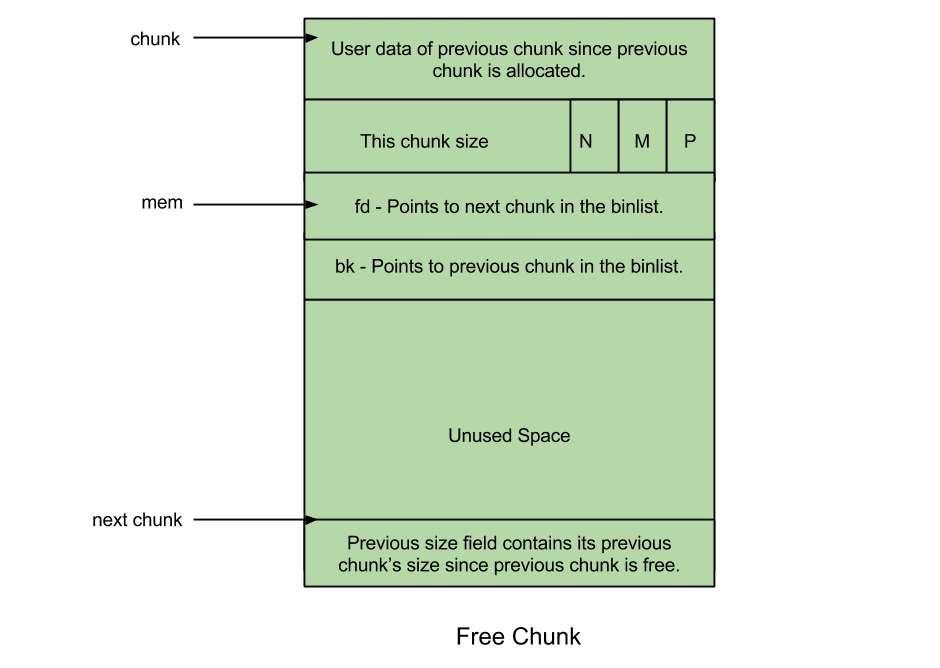
\includegraphics[scale=0.3]{image/chunk.png}
\end{figure}

\section{Arena}

To deal with multiple threads, multiple regions of memory can be active at any given time. Multiple threads can be serviced simultaneously by these regions of memory without blocking each other. A main arena exists which represents the region of memory presented by the initial application heap. Additional arena's are created using mmap as the pressure from threads increase. To make the changes to an arena atomic, each arena possesses a mutex which is acquired by the thread that is using it. \cite{mallocinternals}

\newpage

\begin{lstlisting}
  struct arena {
    chunk_ptr top; /* A pointer to the top chunk */
    chunk_t ubin;  /* Unsorted bin (free list)   */
    chunk_t sbin[SBIN_COUNT]; /* Chunks sized 16, 24,.. 256 spaced 8 bytes*/
    chunk_t bbin[BBIN_COUNT]; /* Log spaced chunks 512,.. (1MiB - 1)*/
    struct arena *next; /* ... */
    struct arena *free; /* ... Part of a linked list of arenas */
    pthread_mutex_t m;  /* For concurrency */
  };
  
\end{lstlisting}

An arena contains a pointer to a top chunk. The top chunk or the wilderness chunk in Doug Lee's Malloc ``represents the space bordering the topmost address allocated by the system''. It can be extended by using sbrk \cite{douglee}. The top chunk is extended when there are no more free chunks of the correct size available.

When a non-mmaped chunk is freed, it is immediately inserted into the unsorted bin list. Freeing memory is very fast. During a myalloc call, if no chunks can be found inside the appropriate small bin, the unsorted bin is sorted. Chunks are removed from it, coallesced and placed into the appropriate bins. This is a form of memoisation.

The small bin is an array of free lists that store chunks of specific sizes ranging from 16, 24, 32, .... up to and including 256 bytes. The chunks are doubly linked so they can be removed from the middle of the list during coallescing.

The large bins is an array of free lists that store chunks of a variety of sizes. The first 32 large bins chunks start at 512 and are 64 bytes apart. The next 16 large bins start at 2560 and are 512 bytes apart. Followed by 8 bins which are 4096 bytes apart, 4 bins of 32768, 2 bins of 262144 and 1 bin of any chunks less than 1Mib. Each large bin stores a range of chunks up to but not including the size of chunks stored in the bin in front of it. This is referred to  as being logarithmically spaced \cite{sploitfun}.

The small bins and large bins are initially empty until the unsorted bin is sorted.

The arena is part of a linked list of arenas which grows are new arenas are created to deal with thread contention.

Finally, for concurrency, each arena possess a mutex. This is required when an arena is acquired for servicing, during which any changes made to the arena must be atomic.

\section{Main Arena and Thread Arena}

The main arena explicitly services the main thread. The main arena is stored statically in the myalloc library. The main arena's top chunk uses the main application heap which is extended using sbrk. The main arena does not use the heapinfo structure.

A thread arena services non main threads. There is an upper limit on the quanitity of thread arenas. I have set this to 4. The quanitity of arenas increases until this upper limit as the number of threads increase, until it reaches the limit. At this point multiple threads are assigned to a each thread arena. In my case, I do not follow Glibc Malloc way of assigning arena's to threads, I simply use modular arithmetic on the thread id. This is a technique to deal with thread contention. Multiple threads can be serviced by different arenas simultaneously which reduces time wasted blocking a thread from acquiring memory. By adding a limit on the number of thread arenas, internal fragmentation is reduced \cite{mallocinternals}.

\section{Thread Arena Heaps}

\begin{lstlisting}
  struct heapinfo {
    arena_ptr arena;
    struct heapinfo *prev;
    size_t hsize;
  };
\end{lstlisting}

Multiple heaps can belong to a single thread arena. A heapinfo structure is embedded at the start of a heap. 

The maximum heap size is allocated using mmap. The memory returned from mmap is marked as PROT\_NONE, except for a small initial part. This is a form of incremental allocation. As more memory is needed, the heap can be grown by the marking the additional memory needed as readable and writable. The memory that has no protection is promised by the operating system, but isn't actually paged until you mark it as readable and writable. Therefore there is no cost for allocating the maximum size of a heap at the start. 

Each heap has a maximum size which is a multiple of 2. In my implementation, I use a trick to return memory from mmap that is aligned to the maximum size of a heap. Any chunk belonging to that heap can be mapped to the heapinfo structure (which is located at the start of the heap) without storing any additional information in the chunk itself. To retrieve the heap which the chunk belongs to you, you simply round the memory address of the chunk down to the nearest multiple of the maximum size of a heap.

Therefore, it can be said that top chunk of that arena keeps track of the most recently allocated heap for that arena.

During the construction of a thread arena, the first heap is constructed and the arena structure is embedded directly above the heapinfo structure. The top chunk for this thread arena then points to the remaining region above.

As memory from the top chunk is taken, the heap grows. When it reaches the maximum size, a new heap is created which belongs to the same thread arena. The previous top chunk is internally freed and inserted into an appropriate free list and the top chunk points to the top chunk of the newly created heap.


\begin{figure}[!htb]
  \caption{A graphic showing thread arenas with multiple heaps taken from \cite{sploitfun}.}
  \center
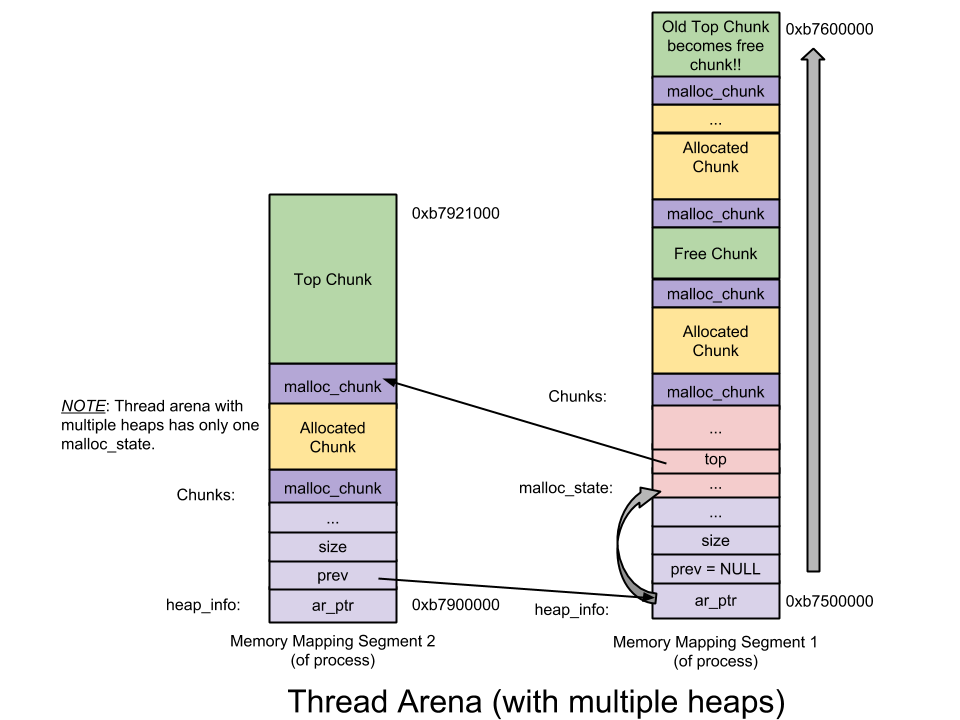
\includegraphics[scale=0.2]{image/threadarenas.png}
\end{figure}

\begin{figure}[!htb]
  \caption{A graphic showing the difference between a main thread arena and a thread arena taken from \cite{sploitfun}.}
  \center
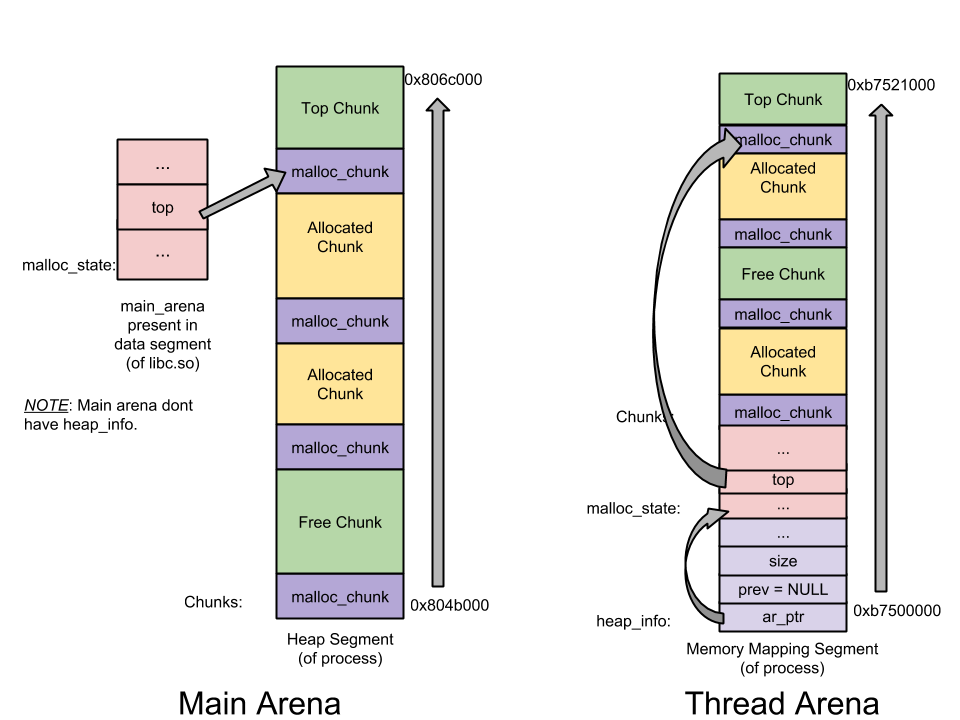
\includegraphics[scale=0.2]{image/mainvsthreadarena.png}
\end{figure}

\begin{figure}[!htb]
  \caption{A graphic showing multiple heaps taken from \cite{mallocinternals}.}
  \center
  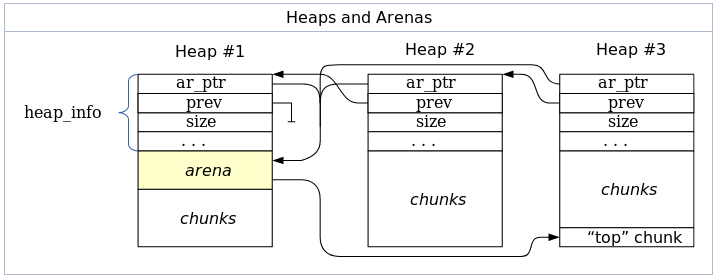
\includegraphics[scale=0.35]{image/multipleheaps.png}
\end{figure}

\newpage

\section{MyAlloc Algorithm}

My algorithm is a simplified version of the algorithm described in \cite{mallocinternals} which is also used by the Glibc Malloc source code \cite{malloc}.

\subsection{MyFree}

If the chunk's ``Is directly mmaped'' bit is set, then munmap it.

A lock to the arena is acquired to which this chunk belongs to which is released at the end.

The chunk is freed by setting the next chunk's ``prev is in use'' bit to off. Coallescing takes place. If the next neighbour chunk is a the top chunk, they are coallesced into a bigger top chunk. Otherwise, the chunk is inserted into the unsorted bin.

\subsection{MyAlloc}

A lock is acquired, myalloc is initialized and this lock is then released.

The size is rounded up to the nearest multiple of 8 greater or equal to the minimum size of a chunk.

If the size is greater or equal to 1MiB, it is directly mmaped.

The arena that services this thread is retrieved or created if it doesn't exist yet, A lock is acquired on this arena and released at the end.

If the chunk is small, try to find a chunk in the appropriate small bin.

Otherwise, start sorting the unsorted bin. If the chunk of the appropriate size is found, split it and return it. While sorting, insert the chunks into their appropriate small and large bins.

If all else fails, split it from the top chunk. The top chunk may by extended to accomodate any additional memory either by sbrk, extending a heap my adding read/write protections or allocating a new heap.

For the chunk that is being returned to the user, it is internally freed by setting the next chunk's ``prev bit in use'' to on.

The chunk is returned to the user.

\section{Conclusion}

I found this practical very enjoyable. It was intriguing to research and discover how other memory allocators the problems associated with memory allocation. Given more time, I would like research how more complex memory allocators work like Jemalloc. Or, how memory allocation in done is different scenarios, for example a slab allocator which caches objects used by kernels or garbage collection in some higher level languages.

\begin{thebibliography}{4}
  
\bibitem{sploitfun} 
Understanding Glibc Malloc,
\\\texttt{https://sploitfun.wordpress.com/2015/02/10/understanding-glibc-malloc/}

\bibitem{douglee} 
A Memory Allocator, by \textit{Doug Lee}
\\\texttt{http://g.oswego.edu/dl/html/malloc.html}


\bibitem{mallocinternals} 
Overview of Malloc,
\\\texttt{https://sourceware.org/glibc/wiki/MallocInternals}

\bibitem{malloc} 
Malloc Source code,
\\\texttt{https://code.woboq.org/userspace/glibc/malloc/malloc.c.html}

\end{thebibliography}


\end{document}
